% !TEX program = xelatex
\documentclass[11pt, a4paper]{article}
\usepackage{graphicx}
\usepackage{tikz}
\usetikzlibrary{shapes.geometric, arrows.meta, positioning}
\usepackage{pgfplots}
\pgfplotsset{compat=1.18}

\begin{document}

\section{Experimental Setup}

% experimental image (placeholder)
\begin{figure}[htbp]
  \centering
  \fbox{\parbox[c][4cm][c]{0.7\textwidth}{\centering Image placeholder: replace with your photo}}
  \caption{Experimental setup for data collection.}
  \label{fig:setup}
\end{figure}

% methodology flowchart
\begin{figure}[htbp]
  \centering
  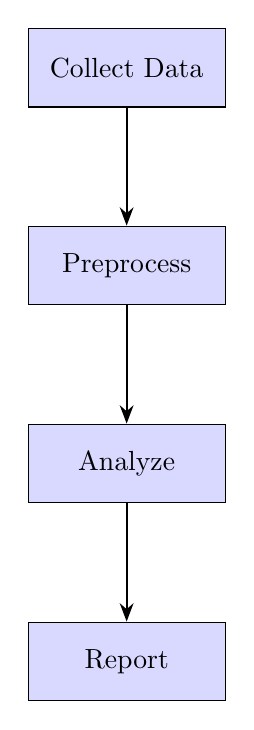
\begin{tikzpicture}[node distance=1.5cm]
    \tikzset{
      process/.style={rectangle, draw, fill=blue!15,
        minimum width=2.5cm, minimum height=1cm, text centered},
      arrow/.style={thick, ->, >=Stealth}
    }
    \node[process] (a) {Collect Data};
    \node[process, below=of a] (b) {Preprocess};
    \node[process, below=of b] (c) {Analyze};
    \node[process, below=of c] (d) {Report};
    \draw[arrow] (a) -- (b);
    \draw[arrow] (b) -- (c);
    \draw[arrow] (c) -- (d);
  \end{tikzpicture}
  \caption{Analysis workflow.}
  \label{fig:workflow}
\end{figure}

% results curve
\begin{figure}[htbp]
  \centering
  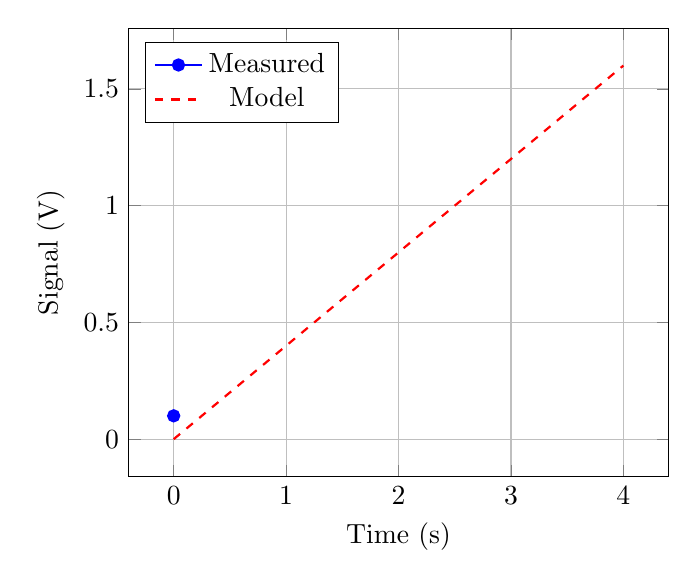
\begin{tikzpicture}
  \begin{axis}[
    xlabel={Time (s)}, ylabel={Signal (V)},
    grid=major, legend pos=north west
  ]
    \addplot[blue, thick, mark=*] table {
      x y
      0 0.1  1 0.3  2 0.7  3 1.2  4 1.5
    };
    \addlegendentry{Measured}
    \addplot[red, dashed, thick, domain=0:4, samples=50] {0.4*x};
    \addlegendentry{Model}
  \end{axis}
  \end{tikzpicture}
  \caption{Measured signal vs.\ theoretical model.}
  \label{fig:results}
\end{figure}

\end{document}
